\documentclass[a6paper]{article}

\usepackage[total={8.9cm,13cm}, top=.8cm, left=.9cm, includefoot]{geometry}
\usepackage{graphicx}

\usepackage[czech]{babel}
\usepackage[utf8]{inputenc}

\usepackage {abstract}


\newcommand*\podpis{\hspace*{0em plus 1fill}\makebox{..........}}

\newcommand \ukol[1]{
	\item
	#1
	\podpis
}
\renewcommand{\abstractname}{ }

%\pagestyle{empty}
\begin{document}


\author {Anpetu}

\title{\textbf{Akičita iyuškin}}
\date{}
\maketitle
\begin{center}
	
{\large
Veselý bojovník
}



\vspace{40pt}
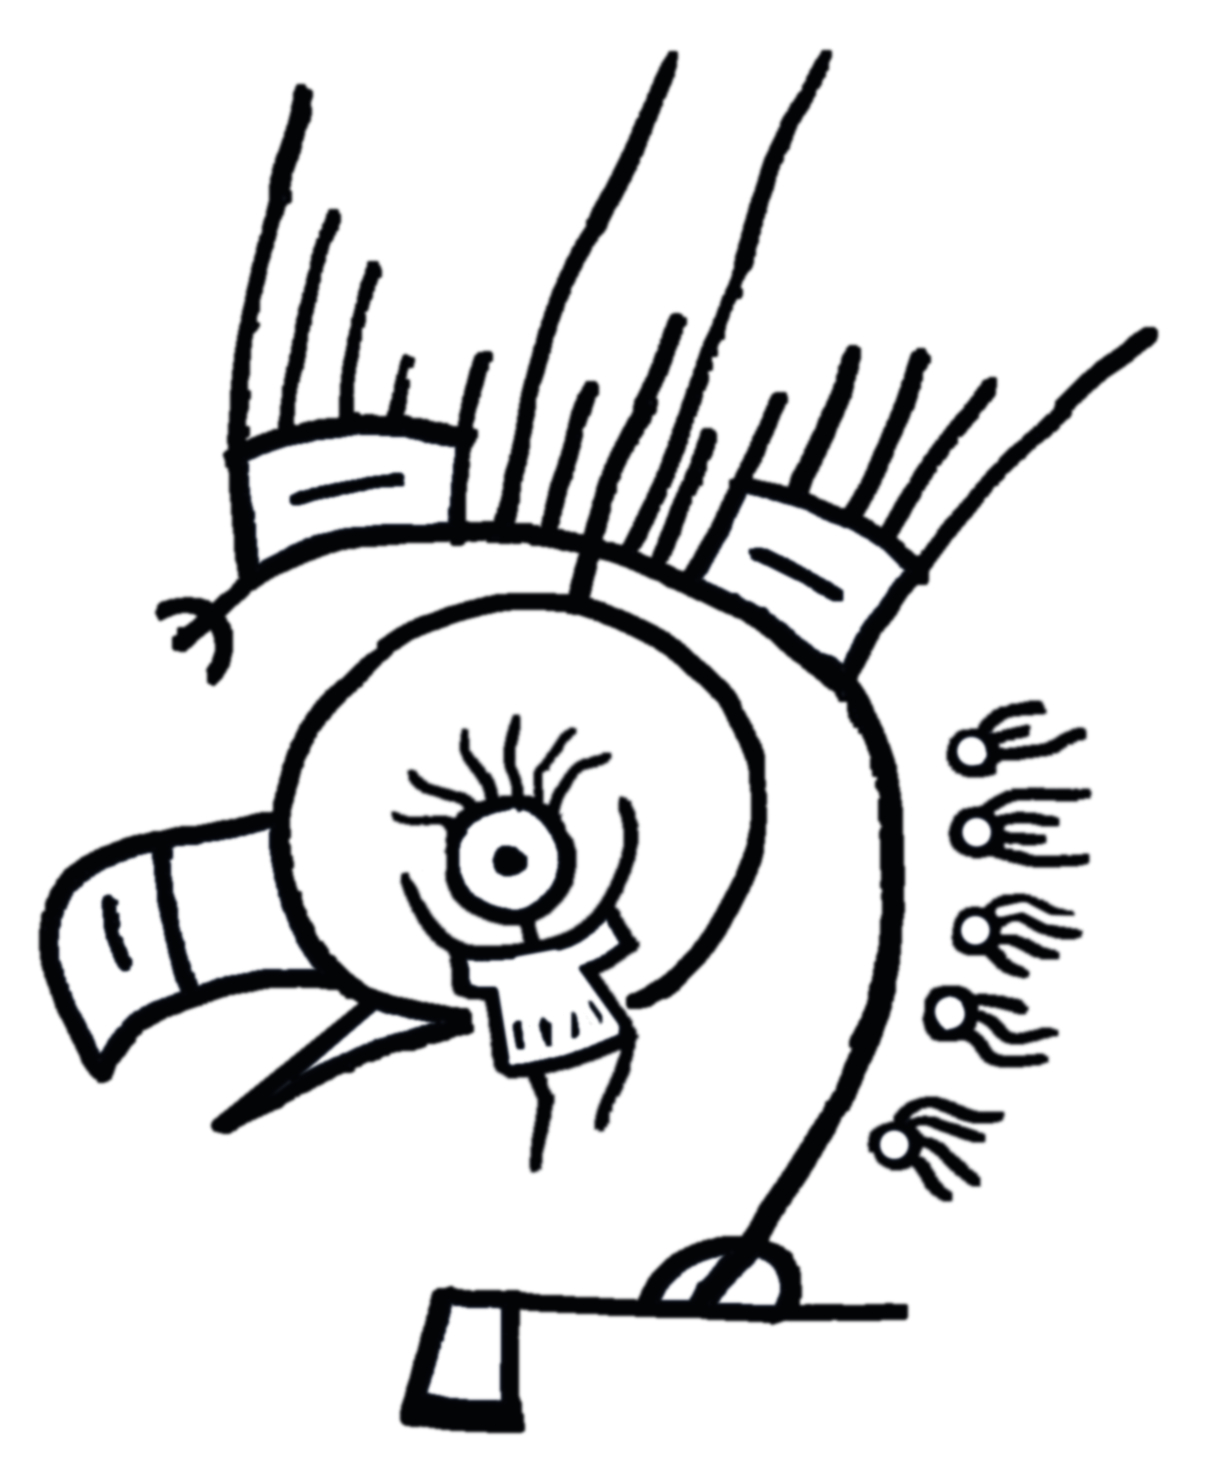
\includegraphics[width=0.5\textwidth]{piktogramy/valecny_orel.jpg}
\end{center}
\clearpage

\vspace*{15 pt}

\begin{Large}
{Bojovnice, bojovníci,}	
\end{Large}


\vspace{12 pt}
\begin{large}
	
Už s námi chvíli putujete a my jsme rádi. Veselý bojovník vám ukáže, co dalšího se můžete ještě vesele naučit.


\vspace{25 pt}

S vašimi udi budete společně plnit úkoly. U každého splněného úkolu vám uďa podepíše políčko vpravo. 

\end{large}

\clearpage

\section*{Zdatnost} % (fold)
\label{sec:zdatnost}
\begin{itemize}
	\ukol{Udělám 10 pořádných kliků}
	\ukol{Učím se plavat, dokážu se udržet nad hladinou}	
	\ukol{Uběhnu kilometr v kuse}
	\ukol{Naučím se stojku}
	\ukol{Celý týden plním cvičící výzvu:	každý den 5 kliků, 30 dřepů a sprchuju/myju se pouze studenou vodou}

\end{itemize}


% section zdatnost (end)

\section*{Zdravověda} % (fold)
\label{sec:zdrav}
\begin{itemize}
	\ukol{Zvládnu zavolat IZS	}
	\ukol{Vím, jak vytáhnout klíště	}
	\ukol{Umím ošetřit popáleninu 1. a 2. stupně	}
	\ukol{Ošetřím kamarádovi zranění	}

\end{itemize}
% section zdrav (end)

\vspace{\fill}
\begin{center}
	
\includegraphics[width=0.4\textwidth]{piktogramy/zajatec_utika.jpg}
\end{center}
\clearpage

\section*{Uzly} % (fold)
\label{sec:uzly}
\begin{itemize}
	\ukol{ Umím liščí smyčku	}
	\ukol{ Zvládnu si uvázat dobráček	}
	\ukol{ Osmičková spojka	}
	\ukol{ Škotova spojka	}
	\ukol{ Zvládnu uvázat autíčka	}
	\ukol{ Napínací zkracovačka	}

\end{itemize}
% section uzly (end)

\section*{Já a svět} % (fold)
\label{sec:ja_a_svet}
\begin{itemize}
	\ukol{Během roku se společně s družinou domluvíme, jakou dobročinnou akci chceme udělat a zrealizujeme ji}

	\ukol{S družinou navštívíme nějakou historickou památku mimo Prahu, vím, kde se nachází a co je na ní zajímavého}

	\ukol{naučím se, jak říct “dobrý den” a “děkuji” a “prosím” ve 3 cizích jazycích}

	\ukol{Vyberu si 3 přísloví, kterým nerozumím, zjistím si, co znamenají a zkusím je nakreslit. Na schůzce je vysvětlím ostatním}

\end{itemize}
% section ja_a_svet (end)

\clearpage

\section*{Skauting a oddíl} % (fold)
\label{sec:skauting}
\begin{itemize}
	\ukol{Vím, kdo založil světový skauting, popíšu, v čem se jeho zakladatelé lišili}
\ukol{Vím, kdo je teď hlavním vedoucím oddílu a jeho zástupcem}
\ukol{Popíšu kroj a vím, kam patří která nášivka}
\ukol{Byl jsem na 2 celoodílových trojdenkách}

\end{itemize}
% section skauting (end)


\section*{Tábornictví} % (fold)
\label{sec:tabor}
\begin{itemize}
	\ukol{Zvládnu rozdělat oheň na 3 sirky }
	\ukol{Postavím přístřešek }
	\ukol{S družinou a vedoucími si postavíme týpí }

\end{itemize}
% section tabor (end)



\vspace{\fill}
\begin{center}
	
\includegraphics[width=0.5\textwidth]{piktogramy/susak_hojnost.jpg}
\end{center}


\clearpage

\section*{Příroda} % (fold)
\label{sec:priroda}
\begin{itemize}
	\ukol{Strávím 15 minut tichým pozorováním přírody, své dojmy zakreslím nebo zapíšu a popíšu je Uďovi}
	\ukol{S družinou navštívíme lesní zoo/oboru, zjistíme si informace o zvěři, kterou tam uvidíme a pak vytvoříme plakát do klubovny}
	\ukol{Vytvořím si herbář, kde bude aspoň 6 rostlin a o každé budu vědět 2 informace}
\item Vyberu si 2 z následujících úkolů:
\begin{itemize}

\ukol{Umím najít na noční obloze 5 souhvězdí}
\ukol{Vytvořím si něco, co každý den používám, z přírodnin}
\ukol{Umím rozeznat 5 stromů podle kůry}
\ukol{Namaluji obraz pouze tím, co najdu v přírodě}
\end{itemize}

\end{itemize}
% section priroda (end)

\vspace{\fill}
\begin{center}
	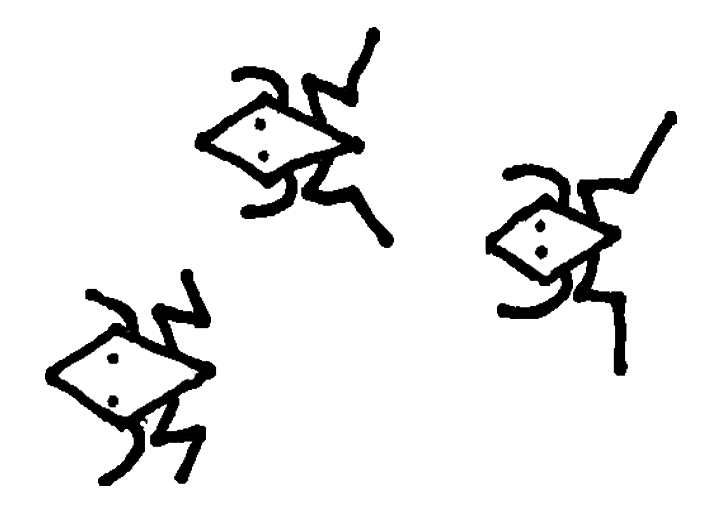
\includegraphics[width=0.5\textwidth]{piktogramy/zabky_nasky.jpg}
\end{center}
\clearpage


\section*{Topografie} % (fold)
\label{sec:topografie}
\begin{itemize}
	\ukol{Znám základní topografické značky a vím co je legenda mapy}
	\ukol{Vím, co jsou vrstevnice}
	\ukol{Dopravím se z bodu A do bodu B za pomoci mapy a buzoly}
	\ukol{Vím, jak se dostanu z domu na Hlavní, Masarykovo a Smíchovské nádraží}
	\ukol{Popíšu a na mapě ukážu cestu z domova do klubovny(Dokázal bych jet na družinovku sám) }

\end{itemize}
% section topografie (end)

\vspace{\fill}
\begin{center}
	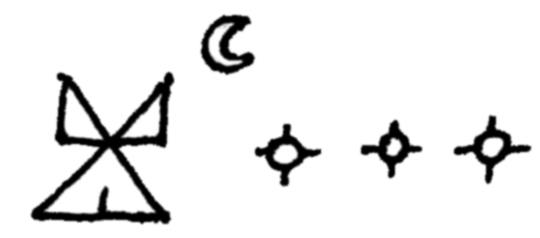
\includegraphics[width=0.5\textwidth]{piktogramy/typko_v_noci.jpg}
\end{center}
\clearpage

\vspace*{50pt}
\begin{center}
	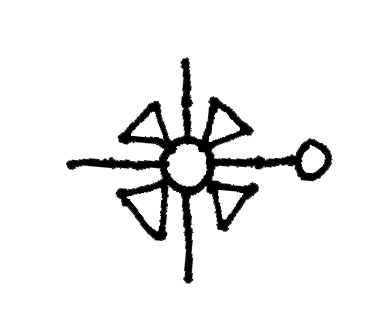
\includegraphics[width=0.5\textwidth]{piktogramy/symbol_1_kdovico.jpg}
\end{center}

\vspace{\fill}

\begin{tiny}
	\hspace{\fill}
	Stezky anpetu, V 1.0RC1
\end{tiny}

\end{document}